\subsection{Observer (观察者)}

\noindent\textbf{意图}

定义对象间的一种一对多的依赖关系,当一个对象的状态发生改变时,所有依赖于它的对象都得到通知并被自动更新。

\textbf{别名}: 依赖(dependent) 发布订阅(publish-subscribe)

\noindent\textbf{动机}

假设有一个人欠了很多钱,债主都盯着这个人的收入。如果这个人有钱了,债主会视该人的经济情况催债。

在这种情况下,这个人的经济情况一旦发生改动,多个债主就会做出相应的动作,这被称作观察者模式。其中关键对象是目标(subject),其他债主是观察者(observer)。

\noindent\textbf{适用性}

\begin{itemize}
    \item 一个抽象模型有两个方面,其中一个方面依赖于另一方面。将这两者封装在独立的对象中,以使它们可以各自独立地改变和复用。
    \item 对一个对象的改变需要同时改变其他对象,而不知道具体有多少对象有待改变。
    \item 一个对象必须通知其他对象,而它又不能假定其他对象是谁。换言之,你不希望这些对象是紧密耦合。
\end{itemize}

\noindent\textbf{结构}

\begin{figure}[H]
    \scriptsize
    \centering
    \begin{tikzpicture}[scale = 1]
        \begin{interface}[text width=2cm]{Subject}{0,0}
            \operation{Attach(Observer)}
            \operation{Detach(Observer)}
            \operation{Notify()}
        \end{interface}
        \begin{class}[text width=2cm]{ConcreteSubject}{0,-3}
            \implement{Subject}
            \attribute{subjectState}
            \operation{GetState()}
            \operation{SetState()}
        \end{class}\
        \begin{interface}[text width=2cm]{Observer}{6,0}
            \operation[0]{Update()}
        \end{interface}
        \begin{class}[text width=2.1cm]{ConcreteObserver}{6,-3}
            \implement{Observer}
            \operation{Update()}
            \attribute{observerState}
        \end{class}
        \draw[umlcd style,fill opacity=0,fill=white,->] (Subject) -- (Observer);
        \draw[umlcd style,fill opacity=0,fill=white,->] (ConcreteObserver) -- (ConcreteSubject);
    \end{tikzpicture}
\end{figure}

\noindent\textbf{参与者}

\begin{itemize}
    \item \textbf{Subject}: 目标知道它的观察者。可以有任意多个观察者观察同一个目标; 提供注册和删除观察者对象的接口。
    \item \textbf{Observer}: 为哪些在目标发生改变时需要获得通知的对象定义一个更新接口。
    \item \textbf{ConcreteSubject}: 将有关状态存入各 ConcreteObserver 对象; 当它的状态发生改变时,向其各个观察者发出通知。
    \item \textbf{ConcreteObserver}: 维护一个指向 ConcreteSubject 对象的引用; 存储有关状态, 这些状态应与目标的状态保持一致; 实现 Observer 的更新接口,以使自身状态与目标的状态保持一致。
\end{itemize}

\noindent\textbf{协作}

\begin{itemize}
    \item 当 ConcreteSubject 发生任何可能导致其观察者与本身状态不一致的改变时,它将通知它的各个观察者。
    \item 在得到一个具体目标的改变通知后, ConcreteObserver 对象可向目标对象查询信息。ConcreteObserver 使用这些信息使它的状态与目标对象的状态一致。
\end{itemize}

\begin{figure}[H] 
    \centering 
    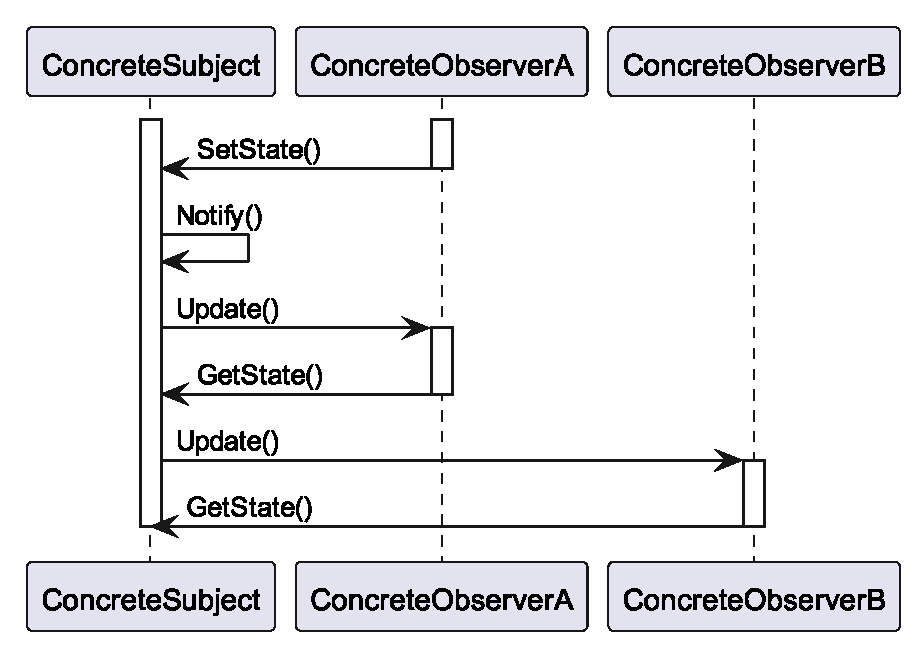
\includegraphics[width=8cm]{figures/Observer.eps} 
\end{figure}

注意发出改变请求的 Observer 对象并不立即更新,而是将其推迟到它从目标得到一个通知之后。Notify 不总是由目标对象调用,它也可被一个观察者或其他对象调用。

\noindent\textbf{优缺点}

\begin{itemize}
    \item \textbf{目标和观察者间的抽象耦合}: 一个目标所知道的仅仅是他有一系列观察者,每个都符合抽象的 Observer 类的简单接口。目标不知道任何一个观察者术语哪个具体的类。这样目标和抽象者之间的耦合是抽象的和最小的。
    \item \textbf{支持广播通信}: 不像通产的请求,目标发送的通知不需要指定它的接收者。通知被自动广播给所有已向该目标对象登记的对象。
    \item \textbf{意外的更新}: 由于一个观察者并不知道其他观察者的存在,它可能对改变目标的最终代价一无所知。
\end{itemize}

\noindent\textbf{例子}

\begin{itemize}
    \item Java: \url{https://blog.csdn.net/itachi85/article/details/50773358}
    \item Video: \url{https://www.bilibili.com/video/BV1vg4y1v7V4}
\end{itemize}

\lstinputlisting[language=Python]{../../scripts/behavioral/Observer.py}

\newpage